% ============================================================================
% Section 6: Consensus Mechanism
% ============================================================================

\section{Consensus Mechanism}
\label{sec:consensus}

\Botho employs a hybrid consensus mechanism combining proof-of-work (PoW)
block proposal with Stellar Consensus Protocol (SCP) finalization. This
achieves permissionless participation with fast deterministic finality.

\subsection{Design Rationale}

\subsubsection{Why Not Pure PoW?}

Nakamoto consensus provides permissionless participation but suffers from:
\begin{itemize}
  \item \textbf{Slow finality}: Probabilistic finality requires multiple
    confirmations (typically 10--60 minutes).
  \item \textbf{Reorg vulnerability}: Transactions can be reversed by chain
    reorganizations, even after confirmation.
  \item \textbf{Energy waste}: Hashpower expended on orphaned blocks provides
    no value.
\end{itemize}

\subsubsection{Why Not Pure BFT?}

Classical BFT protocols provide deterministic finality but require:
\begin{itemize}
  \item \textbf{Known participants}: Fixed validator sets conflict with
    permissionless design.
  \item \textbf{Quadratic messaging}: $O(n^2)$ communication limits
    scalability.
  \item \textbf{Synchrony assumptions}: Liveness depends on network timing
    bounds.
\end{itemize}

\subsubsection{Hybrid Approach}

\Botho combines the strengths of both:
\begin{center}
\begin{tabular}{lcc}
\toprule
\textbf{Property} & \textbf{PoW} & \textbf{SCP} \\
\midrule
Permissionless participation & \checkmark & --- \\
Fair distribution & \checkmark & --- \\
Deterministic finality & --- & \checkmark \\
Fast confirmation & --- & \checkmark \\
Byzantine fault tolerance & --- & \checkmark \\
\bottomrule
\end{tabular}
\end{center}

% Consensus Flow Diagram
% Shows PoW block proposal flowing into SCP finalization
%
% ACCESSIBILITY ALT TEXT:
% A timeline diagram showing Botho's hybrid consensus. On the left, three
% orange boxes represent miners A, B, C proposing blocks via proof-of-work.
% Arrows converge into the SCP finalization phase (blue boxes): Nomination,
% Prepare, Commit. The final green box shows Externalize (Finalized). A time
% arrow at bottom shows progression from t0 (proposals) through t1-t3 to
% deterministic finality. Unlike Bitcoin, finalized blocks cannot be reverted.

\begin{figure}[ht]
\centering
\begin{tikzpicture}[
    node distance=0.8cm and 1.5cm,
    phase/.style={rectangle, draw, rounded corners, minimum width=2cm, minimum height=1cm, align=center, font=\small},
    miner/.style={phase, fill=orange!20},
    scp/.style={phase, fill=blue!20},
    final/.style={phase, fill=green!20},
    arrow/.style={->, >=stealth, thick},
    bigarrow/.style={->, >=stealth, very thick, draw=gray},
]

% PoW Phase
\node[miner] (pow1) {Miner A\\proposes};
\node[miner, below=0.5cm of pow1] (pow2) {Miner B\\proposes};
\node[miner, below=0.5cm of pow2] (pow3) {Miner C\\proposes};

% PoW label
\node[above=0.3cm of pow1, font=\bfseries\small] {PoW Proposals};

% SCP Nomination Phase
\node[scp, right=2cm of pow1] (nom) {Nomination\\Phase};

% SCP Ballot Phase
\node[scp, right=1.5cm of nom] (prep) {Prepare};
\node[scp, right=1cm of prep] (commit) {Commit};

% Externalize
\node[final, right=1.5cm of commit] (ext) {Externalize\\(Finalized)};

% Arrows from miners to nomination
\draw[arrow] (pow1) -- (nom);
\draw[arrow] (pow2) -- (nom);
\draw[arrow] (pow3) -- (nom);

% SCP flow
\draw[arrow] (nom) -- (prep) node[midway, above, font=\scriptsize] {vote};
\draw[arrow] (prep) -- (commit) node[midway, above, font=\scriptsize] {accept};
\draw[arrow] (commit) -- (ext) node[midway, above, font=\scriptsize] {confirm};

% Time arrow at bottom
\draw[bigarrow] (-1,-3) -- (12,-3) node[right, font=\small] {Time};

% Time markers
\node[below=3.2cm of pow2, font=\scriptsize] {$t_0$: Block proposals};
\node[below=3.2cm of nom, font=\scriptsize] {$t_1$: Nomination};
\node[below=3.2cm of $(prep)!0.5!(commit)$, font=\scriptsize] {$t_2$: Ballot};
\node[below=3.2cm of ext, font=\scriptsize] {$t_3$: Final};

% Timing annotation
\node[right=0.5cm of ext, align=left, font=\scriptsize] {Deterministic\\finality\\(no forks)};

% SCP label
\node[above=0.5cm of $(nom)!0.5!(commit)$, font=\bfseries\small] {SCP Finalization};

% Brace for SCP phases
\draw[decorate, decoration={brace, amplitude=5pt, raise=2pt}]
    (nom.north west) -- (commit.north east)
    node[midway, above=8pt, font=\scriptsize] {Quorum agreement};

\end{tikzpicture}
\caption{Hybrid PoW + SCP consensus flow. Multiple miners propose blocks via
proof-of-work (permissionless participation), then SCP achieves deterministic
finality through quorum agreement. Unlike pure PoW, finalized blocks cannot
be reverted---providing instant settlement guarantees.}
\label{fig:consensus-flow}
\end{figure}


\subsection{Stellar Consensus Protocol}
\label{sec:scp}

SCP~\cite{scp} achieves Byzantine agreement with open membership through
\textit{federated Byzantine agreement} (FBA).

\subsubsection{Quorum Slices}

Each node $v$ declares a \textit{quorum slice} $Q(v)$---the set of nodes
$v$ trusts for consensus. Unlike classical BFT where all nodes agree on
membership, SCP allows heterogeneous trust:

\begin{definition}[Quorum Slice]
A quorum slice for node $v$ is a set $Q(v) \subseteq V$ such that $v \in Q(v)$
and $v$ will accept a statement if all nodes in $Q(v)$ accept it.
\end{definition}

\begin{definition}[Quorum]
A set $U \subseteq V$ is a quorum if for every node $v \in U$, there exists
a quorum slice $Q(v) \subseteq U$.
\end{definition}

Informally, a quorum is a set of nodes sufficient for agreement---each member
has ``enough'' trusted nodes within the set to be convinced.

\subsubsection{Quorum Intersection}

Safety requires that any two quorums overlap:

\begin{definition}[Quorum Intersection]
A system has quorum intersection if for all quorums $U_1, U_2$:
$U_1 \cap U_2 \neq \emptyset$.
\end{definition}

\begin{theorem}[SCP Safety]
If the network has quorum intersection and no Byzantine nodes, then SCP
provides safety: no two honest nodes externalize different values for the
same slot.
\end{theorem}

\subsubsection{Tiered Quorum Structure}

\Botho uses a tiered quorum structure balancing decentralization with
robustness:

\begin{lstlisting}[language=,caption={Default quorum slice configuration}]
QuorumSlice {
    // Tier 1: Infrastructure nodes (high-uptime, well-connected)
    threshold: 3,
    validators: [
        "node1.botho.org",
        "node2.botho.org",
        "node3.botho.org",
        "node4.botho.org",
    ],
    // Tier 2: Community validators
    inner_sets: [
        {
            threshold: 2,
            validators: ["community1", "community2", "community3"],
        },
    ],
}
\end{lstlisting}

This requires agreement from 3 of 4 infrastructure nodes AND 2 of 3
community validators, ensuring both stability and decentralization.

% Quorum Slice Structure Diagram
% Venn diagram showing tiered quorum structure with infrastructure and community validators
%
% ACCESSIBILITY ALT TEXT:
% A Venn diagram showing Botho's tiered quorum structure. The outer blue
% ellipse contains 4 infrastructure validator nodes (I1-I4) requiring 3-of-4
% agreement. A smaller green ellipse inside contains 3 community validator
% nodes (C1-C3) requiring 2-of-3 agreement. A dashed red outline shows a
% valid quorum that spans both tiers. The design balances stability from
% infrastructure nodes with decentralization from community participation.

\begin{figure}[ht]
\centering
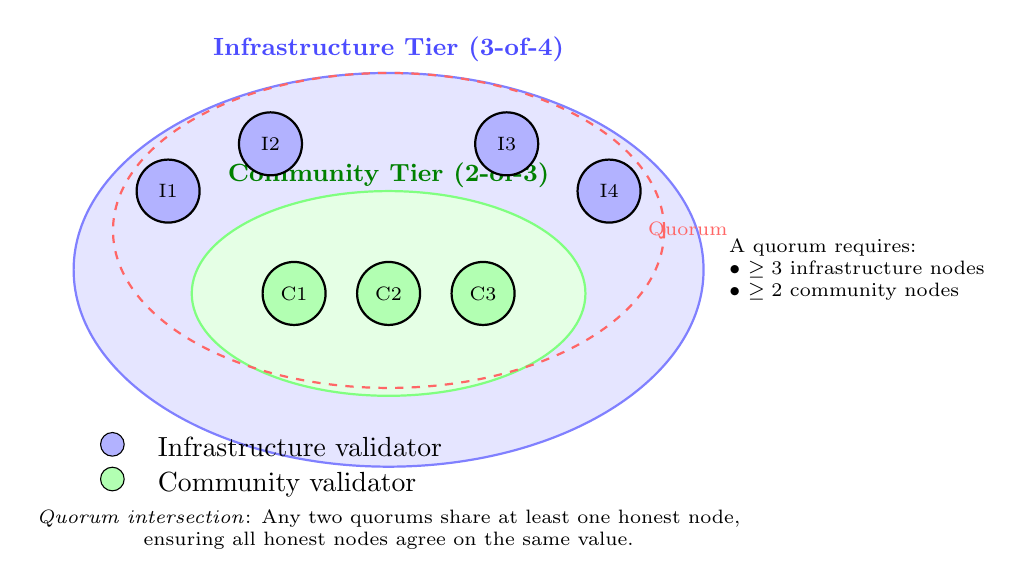
\begin{tikzpicture}[
    node distance=0.8cm,
    validator/.style={circle, draw, minimum size=0.8cm, font=\scriptsize, thick},
    infra/.style={validator, fill=blue!30},
    community/.style={validator, fill=green!30},
    label/.style={font=\small\bfseries},
]

% Infrastructure tier (outer ellipse)
\draw[thick, fill=blue!10, draw=blue!50] (0,0) ellipse (4cm and 2.5cm);
\node[label, blue!70] at (0,2.8) {Infrastructure Tier (3-of-4)};

% Community tier (inner ellipse)
\draw[thick, fill=green!10, draw=green!50] (0,-0.3) ellipse (2.5cm and 1.3cm);
\node[label, green!50!black] at (0,1.2) {Community Tier (2-of-3)};

% Infrastructure nodes
\node[infra] (i1) at (-2.8,1) {I1};
\node[infra] (i2) at (-1.5,1.6) {I2};
\node[infra] (i3) at (1.5,1.6) {I3};
\node[infra] (i4) at (2.8,1) {I4};

% Community nodes
\node[community] (c1) at (-1.2,-0.3) {C1};
\node[community] (c2) at (0,-0.3) {C2};
\node[community] (c3) at (1.2,-0.3) {C3};

% Intersection highlight
\draw[dashed, thick, red!60] (0,0.5) ellipse (3.5cm and 2cm);
\node[font=\scriptsize, red!60] at (3.8,0.5) {Quorum};

% Legend
\node[anchor=west] at (-4,-2.5) {
    \begin{tabular}{ll}
    \tikz\draw[fill=blue!30, draw] (0,0) circle (0.15); & Infrastructure validator \\
    \tikz\draw[fill=green!30, draw] (0,0) circle (0.15); & Community validator \\
    \end{tabular}
};

% Annotations
\node[align=left, font=\scriptsize, anchor=west] at (4.2,0) {
    A quorum requires:\\
    $\bullet$ $\geq 3$ infrastructure nodes\\
    $\bullet$ $\geq 2$ community nodes
};

% Quorum intersection note
\node[align=center, font=\scriptsize] at (0,-3.3) {
    \textit{Quorum intersection}: Any two quorums share at least one honest node,\\
    ensuring all honest nodes agree on the same value.
};

\end{tikzpicture}
\caption{Tiered quorum slice structure in \Botho. Each node's quorum slice requires
agreement from 3-of-4 infrastructure validators AND 2-of-3 community validators.
This design balances network stability (infrastructure tier) with decentralization
(community tier). Quorum intersection is guaranteed when Byzantine nodes are below
threshold.}
\label{fig:quorum-slices}
\end{figure}


\subsection{Consensus Phases}

The consensus process proceeds through four phases for each block slot:

\subsubsection{Phase 1: Block Proposal (PoW)}

Miners compete to propose blocks via proof-of-work:

\begin{enumerate}
  \item Miner constructs candidate block with transactions from mempool
  \item Miner searches for nonce satisfying:
    \begin{equation}
    \Hash(\text{block\_header} \| \text{nonce}) < \text{target}
    \end{equation}
  \item First valid block is broadcast to the network
  \item Multiple proposals may arrive; SCP selects among them
\end{enumerate}

\textbf{Why PoW for proposal?}
\begin{itemize}
  \item \textbf{Permissionless}: Anyone can propose blocks
  \item \textbf{Fair distribution}: Block rewards are distributed by
    computational contribution
  \item \textbf{Sybil resistance}: Creating proposals requires real resources
\end{itemize}

\subsubsection{Phase 2: Nomination}

Nodes nominate candidate values (block hashes) for the slot:

\begin{enumerate}
  \item Node receives valid block proposals
  \item Node nominates the first valid proposal received (tie-breaking by
    lowest hash)
  \item Nodes accept nominations from their quorum slices
  \item Nomination converges to a single candidate when a quorum agrees
\end{enumerate}

\begin{lstlisting}[language=,caption={Nomination message structure}]
NominationMessage {
    slot_index: u64,
    voted: Vec<BlockHash>,      // Values this node votes for
    accepted: Vec<BlockHash>,   // Values this node has accepted
}
\end{lstlisting}

\subsubsection{Phase 3: Ballot Protocol}

Once nomination produces a candidate, nodes run the ballot protocol to
commit to a specific value:

\begin{enumerate}
  \item \textbf{Prepare}: Nodes vote to prepare a ballot $(n, v)$ where
    $n$ is a counter and $v$ is the candidate value
  \item \textbf{Commit}: Once prepared, nodes vote to commit the ballot
  \item \textbf{Abort}: If a ballot cannot progress, nodes abort and try
    a higher ballot number
\end{enumerate}

The ballot protocol ensures:
\begin{itemize}
  \item No two different values can be committed for the same slot
  \item Progress is made despite Byzantine nodes (up to threshold)
  \item Aborted ballots do not block future ballots
\end{itemize}

\subsubsection{Phase 4: Externalize}

When a ballot is committed, nodes externalize the value:

\begin{lstlisting}[language=,caption={Externalize message structure}]
ExternalizeMessage {
    slot_index: u64,
    commit: Ballot,              // The committed ballot
    quorum_set_hash: Hash,       // Proves quorum agreement
}
\end{lstlisting}

Externalization represents deterministic finality---the value cannot be
changed without violating quorum intersection.

\subsection{Block Structure}

\begin{lstlisting}[language=,caption={Block structure}]
Block {
    header: BlockHeader,
    minting_tx: MintingTransaction,
    transactions: Vec<PrivateTransaction>,
    scp_proof: SCPProof,
}

BlockHeader {
    version: u8,
    prev_block_hash: Hash,
    merkle_root: Hash,
    timestamp: u64,
    height: u64,
    difficulty: u64,
    nonce: u64,
    minter_public_key: MLDSAPublicKey,
}

SCPProof {
    slot_index: u64,
    externalize_messages: Vec<ExternalizeMessage>,
    // Sufficient messages to prove quorum agreement
}
\end{lstlisting}

\subsection{Difficulty Adjustment}

\Botho uses a responsive difficulty adjustment algorithm:

\begin{equation}
\text{difficulty}_{n+1} = \text{difficulty}_n \times \frac{T_{\text{target}}}{T_{\text{actual}}}
\end{equation}

where:
\begin{itemize}
  \item $T_{\text{target}}$ is the target block time (dynamically adjusted,
    see Section~\ref{sec:monetary})
  \item $T_{\text{actual}}$ is the actual time for the last adjustment
    window (144 blocks)
\end{itemize}

Adjustments are bounded to $[0.5, 2.0]\times$ per window to prevent
oscillation.

\subsection{Fork Resolution}

Unlike pure PoW where the longest chain wins, \Botho's SCP finalization
makes forks impossible for externalized blocks:

\begin{theorem}[Fork Freedom]
\label{thm:fork-freedom}
If the network has quorum intersection and the Byzantine threshold is
not exceeded, no two honest nodes can externalize different blocks at
the same height.
\end{theorem}

\begin{proof}
We prove by contradiction, following the structure of Mazières'
SCP safety proof~\cite{scp}.

\textbf{Definitions}. Let:
\begin{itemize}
  \item $V$ denote the set of all nodes
  \item $Q: V \to 2^{2^V}$ denote the quorum slice function
  \item $\mathcal{Q} \subseteq 2^V$ denote the set of all quorums
  \item $\text{ext}_v(s)$ denote node $v$'s externalized value for slot $s$
  \item $\mathcal{B} \subset V$ denote Byzantine nodes, $|\mathcal{B}| \leq f$
\end{itemize}

\textbf{Quorum intersection property}. By assumption:
\[
\forall Q_1, Q_2 \in \mathcal{Q}: (Q_1 \setminus \mathcal{B}) \cap (Q_2 \setminus \mathcal{B}) \neq \emptyset
\]
That is, any two quorums share at least one honest node.

\textbf{Ballot protocol invariant}. The SCP ballot protocol maintains
the following invariant for each slot $s$:

\begin{quote}
\emph{Commit Exclusivity}: If honest node $v$ commits ballot $(n, x)$
for slot $s$, then no honest node commits ballot $(n', x')$ for the
same slot with $x' \neq x$ and $n' \leq n$.
\end{quote}

This invariant is established through the prepare phase: a node only
commits $(n, x)$ after confirming that no lower ballot with a different
value can be committed~\cite{scp}.

\textbf{Contradiction argument}. Suppose, for contradiction, that honest
nodes $A$ and $B$ externalize different values for slot $s$ (corresponding
to block height $h$):
\[
\text{ext}_A(s) = b_A \neq b_B = \text{ext}_B(s)
\]

Externalization requires commitment. Let:
\begin{itemize}
  \item $A$ commit ballot $(n_A, b_A)$ with quorum $Q_A \in \mathcal{Q}$
  \item $B$ commit ballot $(n_B, b_B)$ with quorum $Q_B \in \mathcal{Q}$
\end{itemize}

Without loss of generality, assume $n_A \leq n_B$.

By quorum intersection, there exists honest node $C \in (Q_A \setminus \mathcal{B}) \cap (Q_B \setminus \mathcal{B})$.

Node $C$ participated in both quorums. For $C$ to be in $Q_A$, $C$ must
have voted to commit $(n_A, b_A)$. For $C$ to be in $Q_B$, $C$ must have
voted to commit $(n_B, b_B)$.

\textbf{Case 1}: $n_A = n_B$. Node $C$ voted to commit $(n_A, b_A)$ and
$(n_A, b_B)$ with $b_A \neq b_B$. This violates the ballot protocol rule
that honest nodes vote for at most one value per ballot number.
$\Rightarrow$ Contradiction.

\textbf{Case 2}: $n_A < n_B$. For $C$ to vote commit on $(n_B, b_B)$, $C$
must first confirm that no ballot $\leq n_B$ with value $\neq b_B$ is
committed. But $C$ voted to commit $(n_A, b_A)$ with $n_A < n_B$ and
$b_A \neq b_B$. This violates the prepare-before-commit requirement.
$\Rightarrow$ Contradiction.

Both cases yield contradictions. Therefore, our assumption is false,
and no two honest nodes can externalize different values for the same slot.

\textbf{Mapping to block heights}. Each consensus slot corresponds to
exactly one block height. Externalized value = finalized block hash.
Fork freedom at the consensus layer implies fork freedom in the blockchain.

\textbf{Relationship to PoW}. Multiple PoW blocks may be proposed for the
same slot. SCP nomination deterministically selects one candidate before
the ballot protocol begins. The proof above shows the selected candidate
is agreed upon by all honest nodes.
\end{proof}

\begin{corollary}[Finality Irreversibility]
Once a block is externalized at height $h$, no reorganization can replace
it without violating quorum intersection or corrupting $> f$ nodes.
\end{corollary}

\begin{proof}
Reversing externalization at height $h$ requires externalizing a different
block $b'$ for the same slot. By Theorem~\ref{thm:fork-freedom}, this is
impossible under the stated assumptions. An attacker must either:
\begin{enumerate}
  \item Corrupt enough nodes to break quorum intersection, or
  \item Corrupt $> f$ nodes to violate the Byzantine threshold
\end{enumerate}
Both require compromising the network's trust assumptions, not merely
accumulating hashpower (unlike pure PoW).
\end{proof}

\textbf{Handling pre-finalization forks}: Multiple PoW proposals may arrive
before SCP converges. The nomination phase selects a unique winner based on:
\begin{enumerate}
  \item First valid proposal received (per node)
  \item Tie-breaking by lowest block hash
  \item Quorum agreement determines final selection
\end{enumerate}

% Fork Prevention Diagram
% Contrasts Bitcoin's probabilistic finality with Botho's deterministic finality
%
% ACCESSIBILITY ALT TEXT:
% A comparison diagram with two blockchain timelines. Top (Bitcoin): Shows
% a chain with green blocks B1-B3, yellow uncertain blocks B4-B6, and a
% red orphaned fork B3'-B4'. Label indicates 10-60 minute probabilistic
% finality. Bottom (Botho): Shows a single chain of green finalized blocks
% B1-B5 with checkmarks, and one pending block B6. Each block is immediately
% final. Text explains that SCP quorum intersection mathematically prevents
% any alternative history, enabling instant settlement.

\begin{figure}[ht]
\centering
\begin{tikzpicture}[
    node distance=0.6cm,
    block/.style={rectangle, draw, minimum width=1.2cm, minimum height=0.8cm, font=\scriptsize},
    main/.style={block, fill=green!30},
    orphan/.style={block, fill=red!20, draw=red!50},
    pending/.style={block, fill=yellow!20, draw=yellow!50},
    finalized/.style={block, fill=green!50, draw=green!70, thick},
    arrow/.style={->, >=stealth, thick},
]

% === Bitcoin (top) ===
\node[font=\bfseries\small] at (-5.5,3) {Bitcoin (Nakamoto Consensus)};

% Main chain
\node[main] (b1) at (-4,2) {B1};
\node[main] (b2) at (-2.5,2) {B2};
\node[main] (b3) at (-1,2) {B3};
\node[pending] (b4) at (0.5,2) {B4};
\node[pending] (b5) at (2,2) {B5?};
\node[pending] (b6) at (3.5,2) {B6?};

% Fork
\node[orphan] (f1) at (-1,3.2) {B3'};
\node[orphan] (f2) at (0.5,3.2) {B4'};

% Arrows
\draw[arrow] (b1) -- (b2);
\draw[arrow] (b2) -- (b3);
\draw[arrow] (b3) -- (b4);
\draw[arrow] (b4) -- (b5);
\draw[arrow] (b5) -- (b6);
\draw[arrow, red!50] (b2) -- (f1);
\draw[arrow, red!50] (f1) -- (f2);

% Annotations
\node[font=\scriptsize, red!60] at (-0.25,3.8) {Orphaned fork};
\node[font=\scriptsize, align=center] at (2.75,1.2) {Probabilistic finality\\(wait 6+ blocks)};
\draw[decorate, decoration={brace, amplitude=3pt, mirror}]
    (b4.south west) -- (b6.south east)
    node[midway, below=5pt, font=\scriptsize] {Uncertain};

% === Botho (bottom) ===
\node[font=\bfseries\small] at (-5.5,-0.5) {\Botho\ (PoW + SCP)};

% Single chain with finality markers
\node[finalized] (s1) at (-4,-1.5) {B1};
\node[finalized] (s2) at (-2.5,-1.5) {B2};
\node[finalized] (s3) at (-1,-1.5) {B3};
\node[finalized] (s4) at (0.5,-1.5) {B4};
\node[finalized] (s5) at (2,-1.5) {B5};
\node[pending] (s6) at (3.5,-1.5) {B6};

% Finality markers
\foreach \x in {s1,s2,s3,s4,s5} {
    \node[font=\tiny, green!50!black] at ($(\x.south)+(0,-0.3)$) {\checkmark};
}

% Arrows
\draw[arrow] (s1) -- (s2);
\draw[arrow] (s2) -- (s3);
\draw[arrow] (s3) -- (s4);
\draw[arrow] (s4) -- (s5);
\draw[arrow] (s5) -- (s6);

% SCP finalization box
\draw[dashed, thick, blue!50, rounded corners] ($(s6.north west)+(-0.2,0.4)$) rectangle ($(s6.south east)+(0.2,-0.2)$);
\node[font=\scriptsize, blue!50] at (3.5,-0.8) {SCP finalizing};

% No fork annotation
\draw[thick, red, ->] (0.5,-3) -- (0.5,-2.5);
\node[font=\scriptsize, align=center] at (0.5,-3.4) {Fork impossible:\\quorum intersection\\prevents divergence};

% Comparison annotations
\node[align=left, font=\scriptsize, anchor=west] at (5,-0.5) {
    \textbf{Key difference:}\\
    Once SCP externalizes\\
    a block, it cannot be\\
    reverted---even by a\\
    51\% attack.
};

% Timing comparison
\node[align=left, font=\scriptsize] at (-4.5,-3.5) {
    Bitcoin: 10--60 min for ``confidence''\\
    \Botho: 5 sec for \textit{absolute} finality
};

\end{tikzpicture}
\caption{Fork prevention comparison. Bitcoin (top) achieves only probabilistic
finality---transactions can be reversed by reorganizations, requiring multiple
confirmations for confidence. \Botho (bottom) achieves deterministic finality
via SCP: once a block is externalized, quorum intersection mathematically
guarantees no alternative history can exist. This enables instant settlement
with no risk of reversal.}
\label{fig:fork-prevention}
\end{figure}


\subsection{Timing Analysis}

\begin{table}[h]
\centering
\caption{Consensus timing breakdown}
\label{tab:timing}
\begin{tabular}{@{}lr@{}}
\toprule
\textbf{Phase} & \textbf{Time} \\
\midrule
Block proposal (PoW) & Variable (5--40s target) \\
Nomination & $\sim$1s \\
Ballot prepare & $\sim$1s \\
Ballot commit & $\sim$1s \\
Externalize & $<$1s \\
\midrule
\textbf{Total finality} & Block time + $\sim$3--4s \\
\bottomrule
\end{tabular}
\end{table}

In practice, finality occurs within 5 seconds of block proposal, compared
to 10--60 minutes for pure PoW systems.

\subsection{Liveness Guarantees}

\begin{theorem}[SCP Liveness]
If the network is eventually synchronous and at most $f$ nodes are Byzantine
(where each quorum can tolerate $f$ failures), then SCP eventually makes
progress.
\end{theorem}

\textbf{Graceful degradation}: If quorum intersection fails (e.g., due to
network partition), safety is preserved---nodes simply halt rather than
fork. This is a conscious design choice: safety over liveness.

\subsection{Security Properties}

\subsubsection{Byzantine Fault Tolerance}

The system tolerates Byzantine behavior from nodes outside any quorum's
blocking threshold. For the default tier structure:
\begin{itemize}
  \item Infrastructure tier: 1 of 4 can be Byzantine
  \item Community tier: 1 of 3 can be Byzantine
\end{itemize}

\subsubsection{Nothing-at-Stake Resistance}

Unlike pure proof-of-stake systems, PoW proposal ensures:
\begin{itemize}
  \item Proposing multiple blocks requires multiple PoW solutions
  \item Resources are burned regardless of which block is selected
  \item No advantage to ``voting for everything''
\end{itemize}

\subsubsection{Long-Range Attack Resistance}

SCP finality prevents long-range attacks:
\begin{itemize}
  \item Once externalized, blocks cannot be reverted
  \item Rewriting history requires corrupting quorum intersection
  \item No ``weak subjectivity'' bootstrap problem
\end{itemize}

\subsection{Comparison with Alternatives}

\begin{table}[h]
\centering
\caption{Consensus mechanism comparison}
\label{tab:consensus-comparison}
\begin{tabular}{@{}lccc@{}}
\toprule
\textbf{Property} & \textbf{\Botho} & \textbf{Bitcoin} & \textbf{Tendermint} \\
\midrule
Finality & Deterministic & Probabilistic & Deterministic \\
Finality time & $\sim$5--10s & $\sim$60 min & $\sim$6s \\
Permissionless & Yes & Yes & No \\
Fork possible & No & Yes & No \\
Byzantine tolerance & Quorum-based & 50\% hashpower & 1/3 validators \\
Energy efficiency & Medium & Low & High \\
\bottomrule
\end{tabular}
\end{table}

\subsection{Mining Pool Considerations}
\label{sec:mining-pools}

Mining pools aggregate hashpower from multiple miners, distributing rewards
proportionally. \Botho's hybrid consensus requires adaptations to traditional
pooling protocols.

\subsubsection{Pool Protocol Compatibility}

Standard Stratum-style protocols require modification for PoW+SCP:

\begin{lstlisting}[caption={Modified pool work assignment}]
PoolWorkAssignment {
    // Standard PoW fields
    job_id: u64,
    prev_hash: Hash,
    coinbase_template: Vec<u8>,
    merkle_branches: Vec<Hash>,
    target: Difficulty,

    // Botho-specific: SCP context
    slot_index: u64,
    quorum_set_hash: Hash,
    nomination_deadline: Timestamp,
}
\end{lstlisting}

\textbf{Key difference}: Pools must track SCP slot progress and coordinate
work assignments with nomination deadlines. Stale work (missed nomination)
produces no reward even if PoW is valid.

\subsubsection{Block Reward Attribution}

Minting transactions in \Botho include the minter's public key, creating
challenges for pool reward distribution:

\begin{itemize}
  \item \textbf{Pool-controlled keys}: Pool creates minting transaction,
    distributes rewards via separate payment transactions
  \item \textbf{Pay-per-share (PPS)}: Pool pays from reserve for valid shares,
    assumes variance
  \item \textbf{Proportional (PROP)}: Miners receive proportion of actual
    block rewards found
\end{itemize}

\textbf{Cluster tag implications}: Pool-minted coins carry the pool's cluster
tag. Miners receiving payouts inherit blended tags from the pool's operations.

\subsubsection{SCP Participation}

Pools face a choice in SCP participation:

\begin{enumerate}
  \item \textbf{Pool as SCP node}: Pool runs consensus, coordinates with
    quorum. Requires high uptime and expertise.
  \item \textbf{Delegate SCP}: Pool submits valid blocks to SCP-participating
    nodes for finalization. Simpler but adds trust.
\end{enumerate}

Most pools will likely delegate SCP participation to infrastructure nodes
while focusing on PoW coordination.

\subsubsection{Pool Centralization Risks}

Pooled mining creates centralization pressure:

\begin{itemize}
  \item \textbf{Hash rate concentration}: Large pools may approach majority
    hashpower
  \item \textbf{Censorship capability}: Pools could refuse to include certain
    transactions
  \item \textbf{Network attacks}: Colluding pools could attempt consensus
    manipulation
\end{itemize}

\textbf{Mitigations}:
\begin{itemize}
  \item SCP finality requires quorum agreement beyond PoW majority
  \item Transparent pool policies and open-source implementations encouraged
  \item Economic incentives favor decentralization (smaller pools have
    lower variance for participants)
\end{itemize}

\subsubsection{Solo Mining Viability}

Solo mining remains viable under certain conditions:

\begin{table}[h]
\centering
\caption{Solo vs. pool mining trade-offs}
\label{tab:solo-pool}
\begin{tabular}{@{}lcc@{}}
\toprule
\textbf{Factor} & \textbf{Solo} & \textbf{Pool} \\
\midrule
Variance & Very high & Low \\
Cluster purity & 100\% own cluster & Blended with pool \\
Privacy & Maximum & Pool sees hashrate \\
Minimum hashrate & $\sim$1\% network & Any \\
Technical complexity & Higher & Lower \\
\bottomrule
\end{tabular}
\end{table}

\textbf{Recommendation}: Users prioritizing cluster tag purity (to minimize
progressive fees) should consider solo mining despite higher variance.

\subsubsection{Decentralized Pool Alternatives}

P2Pool-style decentralized pools offer middle ground:

\begin{itemize}
  \item \textbf{Share chain}: Miners build separate share chain proving work
  \item \textbf{Trustless payouts}: Block rewards distributed automatically
    based on share chain
  \item \textbf{No central operator}: Removes single point of failure/censorship
\end{itemize}

\textbf{Botho adaptation}: P2Pool would need SCP integration for share chain
finalization. Research and development ongoing.

